% -----------------------------------------------------------------------------
% Fault observability in synthesized cipher circuits.
% Target: IEEE HOST 2026.  Class: IEEEtran conference, 6 pages.
% -----------------------------------------------------------------------------
\documentclass[conference]{IEEEtran}
\IEEEoverridecommandlockouts

% --- packages ---
\usepackage{cite}
\usepackage{amsmath,amssymb,amsfonts,amsthm}
\usepackage{algorithm}
\usepackage{algorithmic}
\usepackage{graphicx}
\usepackage{textcomp}
\usepackage{xcolor}
\usepackage{tikz}
\usetikzlibrary{arrows.meta,positioning,calc,shapes.geometric}
\usepackage{booktabs}
\usepackage{siunitx}
\usepackage{url}
\usepackage{microtype}
\usepackage[hidelinks]{hyperref}

% --- theorem environments ---
\newtheorem{proposition}{Proposition}

% --- macros for consistent terminology ---
\newcommand{\AvgDP}{\textsc{AvgDP}}
\newcommand{\AvgBW}{\textsc{AvgBW}}
\newcommand{\FCpct}{\textsc{FC}\%}
\newcommand{\maj}[1]{\textsc{maj}#1}
\newcommand{\bitflip}{\textsc{bit\_flip}}
\newcommand{\GRANRHO}{-0.85}

% --- title block ---
\title{Fault Observability in FPGA-Mapped Cipher Circuits Synthesized from AIG and MIG Representations}

\author{
\IEEEauthorblockN{Anonymous Submission}
\IEEEauthorblockA{Institution withheld for review}
}

\begin{document}
\maketitle

\begin{abstract}
Recent fault-characterization studies inject single-bit faults at gate
outputs and compare per-vector observability metrics across synthesis
flows. We show that, as commonly applied, these metrics can be
confounded by a variable that is not fault resistance: the granularity
of the gate-level representation. Using 15 cipher primitives from
PRESENT, GIFT, PRINCE, SIMON, Keccak-$\chi$, and Speck/ARX, we compare
truth-table LUT/AOIG, 2-input AIG, and MIG representations under the
same gate-output \bitflip{} model. The apparent benefit of majority
synthesis reverses sign with the baseline: relative to the LUT-style
AOIG baseline, MIG reduces average per-vector detection probability
(\AvgDP{}) by 13.0\% on average; relative to a decomposed-AIG baseline at comparable
small-gate granularity, MIG \emph{increases} \AvgDP{} by 21.4\%, with
no circuit showing a reduction. As a granularity control, we restrict
faults to output-driving gates (the realizable DFA target layer);
target-layer \AvgDP{} $=1.000$ across all three representations,
showing that the all-site difference comes from the interior fault-site
population, not from any change in the attacker-facing output layer. One finding remains
stable across representation: ARX primitives exhibit about $1.9\times$
broader output corruption per detected fault than substitution-based
primitives. We give reporting guidelines for synthesis-flow fault metrics
and release the netlists, campaign scripts, generated tables, and scripts
that check the quoted summary numbers.

\end{abstract}

\begin{IEEEkeywords}
Differential fault analysis, logic synthesis, majority-inverter graph,
gate granularity, fault observability, hardware security.
\end{IEEEkeywords}

\section{Introduction}
\label{sec:introduction}

Differential Fault Analysis recovers cryptographic secrets by inducing
transient faults during cipher execution and comparing corrupted outputs
against correct ones~\cite{biham1997dfa,bareltal2006fault}. A natural
way to characterize a hardware implementation is therefore to inject a
single fault at each gate output and measure how often that fault reaches
a primary output. Recent synthesis-aware fault studies use exactly this
kind of gate-level campaign to compare representations such as LUT
netlists, AND-inverter graphs, majority-inverter graphs, and
technology-mapped FPGA circuits.

This paper asks a simple methodological question: when such a campaign
reports that one synthesis representation has lower per-vector fault
observability than another, how much of the effect is caused by the
logic primitive, and how much is caused by the granularity of the
netlist being measured? The distinction matters. A wide truth-table LUT
that directly drives a primary output contributes one observable fault
site with detection probability one. Decomposing the same function into
many small gates creates many interior sites whose effects can be masked
downstream. A metric averaged over all gate sites can therefore move
substantially even when the realized Boolean function and attacker-facing
target layer have not become more fault resistant.

We evaluate this question on 15 cipher primitives synthesized into three
representations: the LUT-style AOIG baseline produced by Yosys, a
decomposed 2-input AIG as a comparable small-gate control, and a
3-input MIG. All three are subjected to the same single gate-output
\bitflip{} campaign. The resulting observation is narrow but important:
the reported AOIG-to-MIG \AvgDP{} reduction is reproducible, but it
does not survive a decomposed-AIG baseline at comparable granularity.

\subsection*{Contributions}

\begin{itemize}
  \item We show that the AOIG-to-MIG \AvgDP{} reduction reverses sign
        under a decomposed-AIG baseline at comparable small-gate granularity:
        LUT$\to$MIG gives a mean $13.0\%$ reduction, while AIG$\to$MIG
        gives a mean $21.4\%$ increase with $0/15$ circuits reduced.
  \item As a granularity control, we measure target-layer \AvgDP{}
        (faults restricted to output-driving gates). This yields \AvgDP{}
        $=1.000$ across all three representations, consistent with the
        interpretation that the all-site difference comes from interior
        fault-site population mix, not from any change in the
        attacker-facing output layer.
  \item We report one result that survives the controls: ARX primitives exhibit
        approximately $1.9\times$ broader output corruption per detected
        fault than substitution-based primitives across representations.
  \item We release the full artifact: netlists, fault simulator, frozen
        JSON outputs, generated tables/figures, and a script that checks
        the paper's quoted summary numbers.\footnote{Artifact:
        \url{https://github.com/Mrunal321/cipher-fault-observability-study}}
\end{itemize}

The rest of the paper proceeds as follows. \S\ref{sec:background}
summarizes MIG synthesis and DFA observability metrics.
\S\ref{sec:methodology} defines the benchmark, fault model, and
granularity-controlled methodology. \S\ref{sec:results} gives the
baseline-flip result, the invariant target-layer result, and the stable
architecture-level finding. \S\ref{sec:discussion} summarizes
reporting guidance and remaining limits, and \S\ref{sec:conclusion}
concludes.

\section{Background and Related Work}
\label{sec:background}

\subsection{Majority-Inverter Graphs}
\label{sec:background:mig}

A Majority-Inverter Graph (MIG)~\cite{amaru2014mig} is a logic
representation in which every internal node is a 3-input majority
gate $\maj3(a, b, c) = ab \lor bc \lor ac$, with optional
complementation on each input edge. MIG synthesis flows such as the
DAC'19 compatible pipeline of~\cite{amaru2019synth} apply algebraic
rewriting, resubstitution, and refactoring passes that exploit
majority-specific identities to reduce node count and depth.

\subsection{Differential fault analysis and the role of representation}
\label{sec:background:dfa}

Differential Fault Analysis (DFA) was introduced
by Biham and Shamir~\cite{biham1997dfa} as a key-recovery attack
against block ciphers under fault injection. The attacker induces a
fault during an encryption, observes the resulting incorrect output,
and uses the difference between correct and faulty ciphertexts to
constrain the secret key. The seminal AES DFA
of~\cite{piret2003dfa} requires as few as two faulty ciphertexts
under a single-byte fault at the right intermediate position; later
work has extended DFA to most major symmetric ciphers and to a
variety of fault models~\cite{bareltal2006fault, joye2012faultattacks}.

The exploitability of a given fault, and therefore the cost of an
end-to-end DFA attack, depends on three quantitative variables
that are functions not only of the cipher but of its hardware
implementation: the number of distinct fault sites accessible to
the adversary, the per-vector probability that an injected fault
produces a detectable output deviation, and the algebraic structure
of the resulting differences. The first two of these vary with the
synthesis flow. We measure them; we do not address the third.

\subsection{Fault analysis tools and prior characterization}
\label{sec:background:tools}

Pre-silicon fault analysis frameworks evaluate the behavior of
synthesized netlists against a parametrized adversary. SYNFI of
Nasahl et al.~\cite{nasahl2022synfi} performs formal pre-silicon
fault analysis on industrial netlists, focusing on whether
designer-inserted countermeasures survive logic-synthesis
optimization. SCFI of~\cite{nasahl2022scfi} hardens
finite-state-machine control flow against multi-fault attacks.
FIVER~\cite{richter2021fiver} and related tools target similar
goals from different angles.

These tools all start with a single, fixed netlist and characterize
how an attacker can exploit it. Our study is complementary: we hold
the cipher and the FPGA target fixed and vary the synthesis flow,
measuring how the choice of gate-level representation moves the
fault observability metrics that those tools take as input.
We do not address countermeasure design or formal fault verification.

\subsection{Higher-arity majority and AQFP}
\label{sec:background:majn}

The mockturtle library~\cite{soeken2018mockturtle} provides a
\texttt{majority5} generator that decomposes MAJ-5 into four MAJ-3
gates following the construction of~\cite{amaru2014mig}. The
\texttt{aqfp\_network} variant supports native n-ary majority nodes
for Adiabatic Quantum-Flux Parametron (AQFP) targets, where
higher-arity majority is a natural primitive of the cell
library~\cite{takeuchi2014aqfp}. No production
cipher-synthesis flow currently targets MAJ-$n$ as a primitive;
\S\ref{sec:results:majn} discusses why this matters for fault
observability.

\section{Benchmark, Metrics, and Methodology}
\label{sec:methodology}

% =============================================================================
\subsection{Benchmark}
\label{sec:methodology:benchmark}

% Pipeline figure for §3. Shows: cipher BLIF -> three representations ->
% fault campaign -> three measured metrics, plus a side branch for the FPGA
% evaluation. Self-contained tikz block; \input it from §3 inside a figure.

\begin{figure*}[tbp]
  \centering
  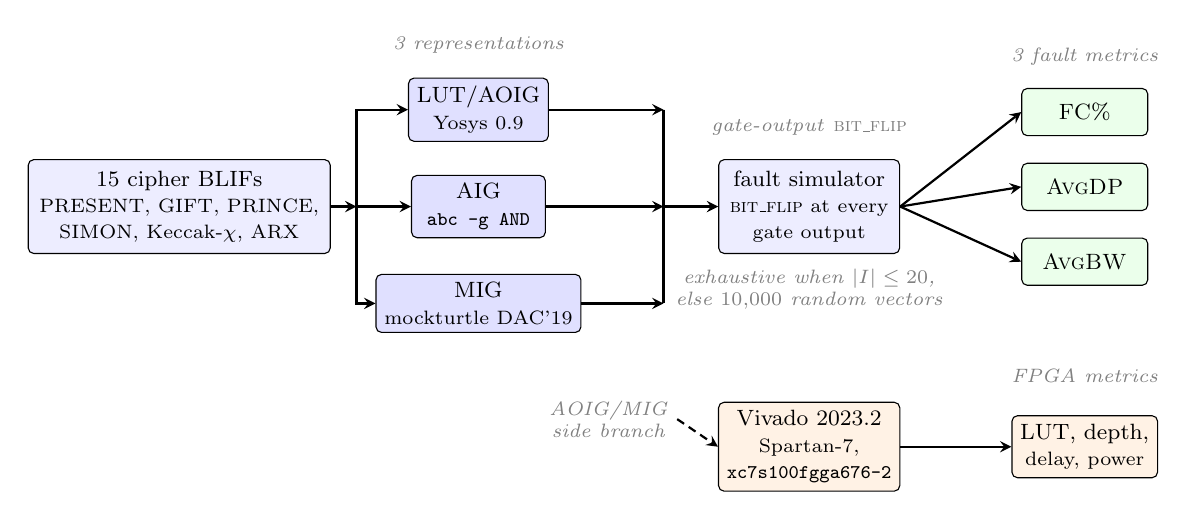
\begin{tikzpicture}[
    >=stealth,
    every node/.style={font=\footnotesize},
    block/.style={draw, rounded corners=2pt, minimum width=2.0cm,
                  minimum height=0.75cm, align=center, fill=blue!7,
                  inner sep=4pt},
    flow/.style={draw, rounded corners=2pt, minimum width=1.7cm,
                 minimum height=0.6cm, align=center, fill=blue!12,
                 inner sep=3pt},
    metric/.style={draw, rounded corners=2pt, minimum width=1.6cm,
                   minimum height=0.6cm, align=center, fill=green!8,
                   inner sep=3pt},
    fpga/.style={draw, rounded corners=2pt, minimum width=1.6cm,
                 minimum height=0.6cm, align=center, fill=orange!10,
                 inner sep=3pt},
    arrow/.style={->, thick},
    bus/.style={thick},
    note/.style={font=\scriptsize\itshape, gray},
  ]

    % ----- INPUT -----
    \node[block] (cipher) at (0, 0) {15 cipher BLIFs\\
        \scriptsize PRESENT, GIFT, PRINCE,\\
        \scriptsize SIMON, Keccak-$\chi$, ARX};

    % ----- THREE REPRESENTATIONS -----
    \node[flow] (aoig) at (3.8,  1.23) {LUT/AOIG\\\scriptsize Yosys 0.9};
    \node[flow] (aig)  at (3.8,  0.00) {AIG\\\scriptsize \texttt{abc -g AND}};
    \node[flow] (mig)  at (3.8, -1.23) {MIG\\\scriptsize mockturtle DAC'19};

    \coordinate (split) at (2.25, 0);
    \draw[arrow] (cipher.east) -- (split);
    \draw[arrow] (split) |- (aoig.west);
    \draw[arrow] (split) |- (aig.west);
    \draw[arrow] (split) |- (mig.west);

    % ----- COMMON FAULT CAMPAIGN -----
    \node[block] (sim) at (8.0, 0) {fault simulator\\
        \scriptsize \textsc{bit\_flip} at every\\
        \scriptsize gate output};

    \coordinate (faultbus) at (6.15, 0);
    \draw[bus] (faultbus |- aoig.east) -- (faultbus |- mig.east);
    \draw[arrow] (aoig.east) -- (faultbus |- aoig.east);
    \draw[arrow] (aig.east) -- (faultbus |- aig.east);
    \draw[arrow] (mig.east) -- (faultbus |- mig.east);
    \draw[arrow] (faultbus) -- (sim.west);

    % ----- METRICS -----
    \node[metric] (fc)   at (11.5,  1.2) {\FCpct};
    \node[metric] (avgdp) at (11.5, 0.25) {\AvgDP};
    \node[metric] (avgbw) at (11.5, -0.7) {\AvgBW};

    \draw[arrow] (sim.east) -- (fc.west);
    \draw[arrow] (sim.east) -- (avgdp.west);
    \draw[arrow] (sim.east) -- (avgbw.west);

    % ----- FPGA SIDE-CAMPAIGN -----
    \node[fpga] (vivado) at (8.0, -3.05) {Vivado 2023.2\\
        \scriptsize Spartan-7,\\
        \scriptsize \texttt{xc7s100fgga676-2}};
    \node[fpga] (fpga_metrics) at (11.5, -3.05) {LUT, depth,\\
        \scriptsize delay, power};

    \node[note, align=center] (fpga_src) at (5.45, -2.7)
      {AOIG/MIG\\side branch};
    \draw[arrow, densely dashed] (fpga_src.east) -- (vivado.west);
    \draw[arrow] (vivado.east) -- (fpga_metrics.west);

    % ----- LABELS -----
    \node[note] at (3.8, 2.05) {3 representations};
    \node[note] at (8.0, 1.0) {gate-output \textsc{bit\_flip}};
    \node[note] at (11.5, 1.9) {3 fault metrics};
    \node[note] at (11.5, -2.15) {FPGA metrics};

    % ----- TEST-VECTOR ANNOTATION -----
    \node[note, align=center] at (8.0, -1.05)
      {exhaustive when $|I| \le 20$,\\else $10{,}000$ random vectors};

  \end{tikzpicture}
  \caption{Measurement pipeline. Each of 15 cipher BLIFs is synthesized
  through three logical representations. The fault simulator injects a single \bitflip{}
  at every gate output of every netlist on every test vector
  (exhaustive when feasible; $10{,}000$ uniform random vectors
  otherwise), producing all-site and target-layer metrics
  (\FCpct{}, \AvgDP{}, \AvgBW). The FPGA side-branch reports LUT,
  depth, delay, and power for context on AOIG/MIG; the fault
  analysis is independent of FPGA tooling.}
  \label{fig:pipeline}
\end{figure*}

Fig.~\ref{fig:pipeline} sketches the full measurement pipeline.

We selected 15 cipher primitives spanning six architecture families:
four 4-bit S-boxes (PRESENT, GIFT, PRINCE, PRINCE$^{-1}$); three
substitution round functions (GIFT \texttt{subcells}, GIFT round,
PRESENT round); one permutation primitive (PRINCE $M'$); two SIMON
round functions (SIMON-32, SIMON-64); two Keccak-$\chi$ widths
(5-bit, 64-row); and three ARX primitives (Speck-32, SpecKey,
MARX-2). Input width ranges from 4 to 1280 bits. FPGA-oriented
AOIG/MIG metrics are included in the artifact for context, but
the fault-analysis claims below use the BLIF-level campaigns.

We analyze three logical representations, all derived from the same raw
cipher BLIF. \emph{LUT/AOIG} is the raw BLIF emitted by Yosys 0.9 from
the cipher's behavioral description, dominated by LUT-style truth-table
primitives. \emph{AIG} is a decomposed 2-input AND-inverter graph, used as a
comparable small-gate granularity control.
\emph{MIG} is a strict 3-input majority-inverter network produced with
the mockturtle logic-synthesis library~\cite{soeken2018mockturtle}. The
exact passes for the AIG and MIG flows are given in
\S\ref{sec:methodology:recipes}; the raw BLIFs and the synthesis driver
are in the artifact.

% =============================================================================
\subsection{Synthesis recipes}
\label{sec:methodology:recipes}

Because our central claim is that fault metrics depend on the gate-level
representation, the exact transformation from the common source BLIF to
each representation is part of the methodology. All three start from the
identical Yosys-emitted truth-table BLIF.

\textit{AIG.} We decompose the source BLIF into a 2-input AND-inverter
graph with Yosys and ABC, using the script
\texttt{read\_blif; hierarchy -auto-top; flatten; proc; techmap; opt;
abc -g AND; opt\_clean; write\_blif}. The \texttt{abc -g AND} step maps
all logic onto 2-input \textsc{and} nodes with inverter edges; no
optimization beyond \texttt{opt}/\texttt{opt\_clean} is applied. This
control exists only to provide a comparable small-gate fault-site
population for comparison with the MIG.

\textit{MIG.} We read the source BLIF into a $k$-LUT network and convert
it to an MIG by NPN node resynthesis
(\texttt{node\_resynthesis} with \texttt{mig\_npn\_resynthesis}). We then
apply a fixed DAC'19-style majority optimization recipe implemented with
stock mockturtle passes~\cite{amaru2019synth}: algebraic depth rewriting,
MIG resubstitution, cut rewriting with MIG NPN resynthesis, and
refactoring. In the artifact, this recipe is selected with
\texttt{--mode=area --mig-flow=dac19\_compat}; the option is used only
to reproduce the mockturtle flow. The resulting netlists are strict
3-input majority-inverter graphs.

% =============================================================================
\subsection{Metrics}
\label{sec:methodology:metrics}

We measure \emph{fault observability}: after flipping one gate-output
bit, does any primary output change, and if so, how often and by how
many bits? This is not a full key-recovery metric. It is a gate-level
description of how injected faults reach the circuit outputs.

Let $C$ have primary inputs $I$, primary outputs $O$, and internal
signals $G(C)$. Let $\mathcal{P}$ be the test-vector set (exhaustive
when $|I| \le 20$, otherwise $10{,}000$ uniform random vectors with
fixed seed). For each fault site $g \in G(C)$ and each vector
$P \in \mathcal{P}$, let $\text{out}(P)$ denote the fault-free primary
outputs and $\text{out}_g(P)$ the primary outputs when $g$ is subject
to a single \bitflip{}. We report three metrics.

\textit{Fault coverage} \FCpct{} asks how many gate-output sites are
ever visible at the primary outputs. A site is detectable if at least
one tested vector makes the faulty output differ from the fault-free
output:
$|\{g : \exists P,\ \text{out}_g(P) \ne \text{out}(P)\}| / |G(C)|$.

\textit{Average per-vector detection probability} \AvgDP{} asks how
often a detectable site is visible. For a site $g$, $\text{dp}(g)$ is
the fraction of tested vectors on which flipping $g$ changes the
primary output. \AvgDP{} averages this value across detectable sites:
$\AvgDP(C) = \frac{1}{|\{g~\text{detectable}\}|} \sum_g \text{dp}(g)$,
where $\text{dp}(g) = |\{P : \text{out}_g(P) \ne \text{out}(P)\}| / |\mathcal{P}|$.
For example, if a fault changes the output on 8 of 16 exhaustive input
vectors, then $\text{dp}(g)=0.5$.

\textit{Average breadth} \AvgBW{} asks how large the visible corruption
is. For every event where the faulty output differs from the correct
output, we count the primary-output Hamming distance. \AvgBW{} is the
mean of those distances over all detecting events.

These metrics vary independently. A circuit can have higher \FCpct{}
than another while having lower \AvgDP{}: more fault sites are
theoretically observable, but each is observed on a smaller share of
input space.

For the granularity-controlled analysis, we compute each metric over two
fault-site populations. The \emph{all-site} population includes every
gate-output site in the representation. This is the common campaign
design, but it is representation-sensitive because decomposing one
Boolean function into many small gates changes both the number and
location of sites being averaged. The \emph{target-layer} population
includes only gates that directly drive primary outputs. This is not a
complete physical fault model, but it is a realizable combinational DFA
target layer and removes the interior-node mix introduced by different
decompositions. Full definitions are in the artifact's
\texttt{paper/metrics.md}.

% =============================================================================
\subsection{Fault model and simulator}
\label{sec:methodology:simulator}

We adopt a single-fault model: the adversary injects one
\bitflip{} at one gate-output wire of the combinational netlist per
evaluation and observes the resulting primary outputs. We do not
model multi-bit faults, transistor-level effects, glitch injection,
delay faults, or end-to-end key-recovery attacks; these are
out of scope.

Our simulator parses BLIF, builds per-gate truth-table lookups, and
evaluates the netlist on all $|\mathcal{P}|$ vectors as a single
vectorized \texttt{numpy.uint8} array. For each gate $g$, the
fault-free signal value $v_g(P)$ is computed once; the faulty
evaluation re-runs propagation with the override
$g \mapsto v_g(P) \oplus 1$. The campaign re-runs full propagation for
each fault site across all test vectors in a vectorized batch; for
the largest circuit (\texttt{keccak\_chi\_64row}, 1602 gates,
$10{,}000$ vectors) it completes in approximately one minute on a
single core.

% =============================================================================
\subsection{Granularity-controlled assessment procedure}
\label{sec:methodology:procedure}

The assessment has three checks. First, we compute all-site \AvgDP{}
for each representation and compare the same MIG netlists against both
the LUT/AOIG baseline and the decomposed-AIG baseline. Second, we
measure the Spearman rank association between all-site \AvgDP{} and
decomposition granularity (fault sites per primary output). Third, we
repeat the campaign on the target-layer population only. These checks
allow us to separate representation-dependent all-site behavior from
behavior that remains stable under controlled fault-site populations.
Results are reported in \S\ref{sec:results}.

% =============================================================================
\subsection{Mechanism: how masking arises}
\label{sec:methodology:mechanism}

The LUT-to-MIG \AvgDP{} change in \S\ref{sec:results:granularity}
has a concrete gate-level mechanism, but the mechanism is a site-mix
effect, not evidence that majority logic is intrinsically more
fault resistant. A \bitflip{} at the output of
gate $g$ is, by definition, observable at $g$ itself because the fault
and the output are the same wire. The question is whether the flipped
value reaches a primary output, which depends entirely on $g$'s
downstream consumers.

For a 3-input majority gate $h$ that consumes $g$ along with two
other inputs $a$ and $b$, the output of $h$ is $1$ iff at least two of
its three inputs are $1$. The vote is \emph{determined} by $a$ and
$b$ alone when $a = b$: $h$'s output is fixed at that shared value
regardless of the third input. We call this the \emph{non-controlling
pattern at $h$ relative to $g$}, in keeping with the ATPG term. When
the other two inputs disagree, $a \ne b$, the third input casts the
deciding vote, and a flip at $g$ propagates through $h$.

Under a uniform distribution over $h$'s other two inputs, the
non-controlling pattern holds with probability $\frac{1}{2}$.
A fault at $g$ that has no downstream consumer other than $h$ therefore
has $\text{dp}(g) = \frac{1}{2}$ in the limit. A LUT-style AOIG
representation often contributes one wide output-adjacent fault site
with $\text{dp}=1$, whereas MIG and AIG decompositions contribute many
interior sites whose downstream consumers can mask them. The all-site
average therefore changes when the representation changes. The central
question in \S\ref{sec:results:granularity} is whether the sign of that
change survives when the baseline is decomposed to comparable
granularity.

% =============================================================================
\subsection{Worked example}
\label{sec:methodology:trace}

We make the mechanism concrete on the \texttt{present\_sbox} MIG
netlist. Gate $g = \texttt{new\_n12}$ is a 3-input majority of
\texttt{pi1}, \texttt{pi2}, and an internal signal \texttt{new\_n11}.
$g$ has exactly one downstream consumer, $h = \texttt{new\_n15}$,
which is a 3-input majority over \texttt{new\_n10}, the complement of
$g$'s value, and \texttt{new\_n14}.
Figure~\ref{fig:masking-example} shows the structure;
Table~\ref{tab:masking-trace} enumerates the per-vector behavior.

% Worked masking example: present_sbox MIG
% Fault site g = new_n12 (MAJ3 of pi1, pi2, new_n11)
% Downstream gate h = new_n15 (MAJ3 of new_n10, ~new_n12, new_n14)
% g has exactly one consumer (h), so dp(g) is determined entirely by h's masking.

\begin{figure*}[tbp]
  \centering
  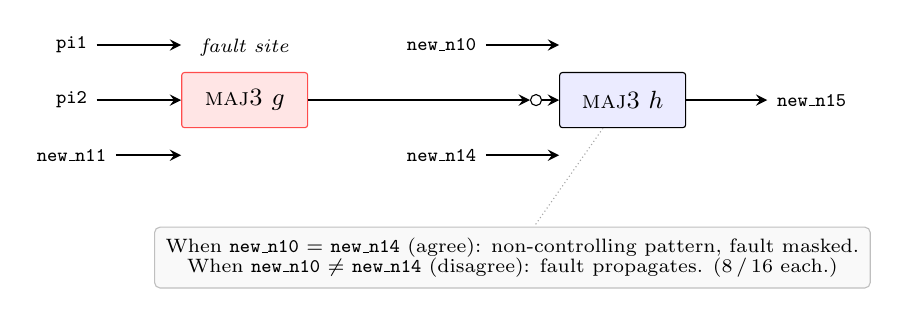
\begin{tikzpicture}[
    >=stealth,
    every node/.style={font=\small},
    gate/.style={draw, rounded corners=1pt, minimum width=1.6cm,
                 minimum height=0.7cm, fill=blue!8},
    fgate/.style={draw, rounded corners=1pt, minimum width=1.6cm,
                  minimum height=0.7cm, fill=red!10, draw=red!70},
    wire/.style={->, thick},
    inv/.style={circle, inner sep=0pt, minimum size=4pt, draw, fill=white},
  ]
    % Primary inputs feeding g
    \node (pi1)   at (-3.2,   1.0) {\scriptsize \texttt{pi1}};
    \node (pi2)   at (-3.2,   0.3) {\scriptsize \texttt{pi2}};
    \node (n11)   at (-3.2,  -0.4) {\scriptsize \texttt{new\_n11}};

    % Fault gate g
    \node[fgate] (g) at (-1.0, 0.3) {\textsc{maj3} $g$};
    \node[above=2pt of g, font=\scriptsize\itshape] {fault site};

    \draw[wire] (pi1) -- (g.west |- pi1);
    \draw[wire] (pi2) -- (g.west);
    \draw[wire] (n11) -- (g.west |- n11);

    % Other inputs to h
    \node (n10)   at (1.5,  1.0) {\scriptsize \texttt{new\_n10}};
    \node (n14)   at (1.5, -0.4) {\scriptsize \texttt{new\_n14}};

    % Downstream gate h (sole consumer of g)
    \node[gate] (h) at (3.8, 0.3) {\textsc{maj3} $h$};

    % Inverter bubble on g -> h edge (h treats g's contribution complemented)
    \node[inv] (bubble) at (2.7, 0.3) {};

    \draw[wire] (g.east) -- (bubble.west);
    \draw[wire] (bubble.east) -- (h.west);
    \draw[wire] (n10) -- (h.west |- n10);
    \draw[wire] (n14) -- (h.west |- n14);

    % Output
    \node (out) at (6.2, 0.3) {\scriptsize \texttt{new\_n15}};
    \draw[wire] (h.east) -- (out.west);

    % Annotation: masking rule
    \node[align=center, font=\scriptsize, draw=gray!50,
          rounded corners=2pt, fill=gray!5, inner sep=4pt]
      (note) at (2.4, -1.7)
      {When \texttt{new\_n10} $=$ \texttt{new\_n14} (agree): non-controlling pattern, fault masked.\\[-1pt]
       When \texttt{new\_n10} $\neq$ \texttt{new\_n14} (disagree): fault propagates. (8\,/\,16 each.)};
    \draw[densely dotted, gray!70] (h) -- (note);
  \end{tikzpicture}
  \caption{Worked masking example from the \texttt{present\_sbox} MIG.
    Gate $g$ (fault site) feeds a single downstream MAJ3 gate $h$
    through a complemented edge. A bit-flip at $g$ propagates to $h$'s
    output iff the other two inputs of $h$ \emph{disagree}; when they
    \emph{agree}, they form the non-controlling pattern and mask the
    fault. Over the 16 exhaustive input vectors, the other two inputs
    agree on 8 vectors (fault masked) and disagree on 8 (fault propagates). Because $g$ has $h$ as its sole consumer, this
    completely determines $g$'s observability: $\mathrm{dp}(g) = 8/16
    = 0.5$. The per-vector trace in Table~\ref{tab:masking-trace}
    enumerates all 16 vectors.}
  \label{fig:masking-example}
\end{figure*}

% Summary of the exhaustive per-vector masking trace for present_sbox.

\begin{table}[tbp]
  \centering
  \caption{Worked-example trace summary. The fault at $g$ is masked when
  the other two inputs of $h$ agree and propagates when they disagree.}
  \label{tab:masking-trace}
  \footnotesize
  \setlength{\tabcolsep}{3.5pt}
  \begin{tabular}{@{}p{0.29\columnwidth}c p{0.28\columnwidth}p{0.23\columnwidth}@{}}
    \toprule
    Other inputs of $h$ & Vectors & Effect at $h$ & Outcome \\
    \midrule
    Agree, $a=b$ &
    $8/16$ &
    Output fixed by $a,b$ &
    Fault masked \\
    Disagree, $a\ne b$ &
    $8/16$ &
    Fault input is decisive &
    Propagates \\
    \midrule
    \multicolumn{3}{@{}l}{Detected vectors for fault at $g$} &
    $8/16$ \\
    \multicolumn{3}{@{}l}{Detection probability $\mathrm{dp}(g)$} &
    $0.5$ \\
    \bottomrule
  \end{tabular}
\end{table}


Over the $2^4 = 16$ exhaustive input vectors, the other two inputs
of $h$ agree on exactly 8 vectors. On those 8 vectors, $h$'s output is
fixed by \texttt{new\_n10} and \texttt{new\_n14}, and the flip at $g$
does not propagate. On the other 8 vectors, \texttt{new\_n10} and
\texttt{new\_n14} disagree, $h$'s output tracks $g$'s value, and the
flip propagates to a primary output. The measured $\text{dp}(g)$ is
$8/16 = 0.5$, exactly the predicted MAJ-3 per-input non-controlling
rate.

This example does not establish a representation-level security
advantage. It shows that downstream majority masking exists and is
identifiable at the gate level. The granularity-controlled
results in \S\ref{sec:results:granularity} show why this local mechanism
must be interpreted together with the distribution of fault sites created
by the synthesis flow.

% =============================================================================
\subsection{Hardware target and reproducibility}
\label{sec:methodology:fpga}

For the FPGA side data included in the artifact, we synthesized each
circuit on a Xilinx Spartan-7 \texttt{xc7s100fgga676-2}
using Vivado 2023.2 with \texttt{synth\_design -flatten\_hierarchy
rebuilt}. Each LUT1 inverter is annotated \texttt{DONT\_TOUCH = TRUE}
post-synthesis to preserve inverter visibility in the LUT histogram;
the target clock period is 10\,ns. The fault-analysis path of the
paper does not depend on FPGA tooling; the post-optimization BLIFs
are included in the artifact and the fault metrics are reproducible
from them on a stock Python 3.10 with NumPy installation.

The accompanying artifact contains the cipher BLIFs,
the synthesized netlists, the fault simulator, the table and figure
generators, and a verification script that checks the quoted summary
numbers against the raw JSON outputs.

\section{Results}
\label{sec:results}

We report three results. First, the all-site \AvgDP{} comparison
reverses sign when the LUT baseline is replaced by a decomposed-AIG
baseline at comparable small-gate granularity. Second, target-layer
\AvgDP{} is invariant across the three representations. Third, the
ARX-versus-substitution \AvgBW{} gap is stable across the representation
controls. We close with the synthetic MAJ-$n$ experiment as a
forward-looking mechanism study.

% =============================================================================
\subsection{The AOIG-to-MIG comparison depends on granularity}
\label{sec:results:granularity}

The original LUT/AOIG-to-MIG comparison is reproducible: on the 15
circuits, all-site \AvgDP{} changes by a mean of $-13.0\%$, with
$13/15$ circuits showing lower \AvgDP{} under MIG. This number is not
wrong, but it is not stable. When the baseline is a decomposed 2-input
AIG at comparable small-gate granularity, the sign reverses: AIG$\to$MIG changes all-site \AvgDP{}
by a mean of $+21.4\%$, and no circuit shows a reduction.
Table~\ref{tab:granularity_confound} lists both comparisons.

\begin{table}[t]
\centering
\caption{All-site \AvgDP{} change (\%) from AOIG to MIG by baseline.
         Negative = MIG has lower \AvgDP{}; positive = MIG has higher.}
\label{tab:granularity_confound}
\footnotesize
\begin{tabular}{@{}lrr@{}}
\toprule
Circuit & LUT$\!\to\!$MIG & AIG$\!\to\!$MIG \\
\midrule
\multicolumn{3}{@{}l}{\textit{4-bit S-box}} \\
\quad PRESENT S-box       & $-21.5$ & $+7.6$  \\
\quad GIFT S-box          & $-16.8$ & $+8.3$  \\
\quad PRINCE S-box        & $-23.7$ & $+9.2$  \\
\quad PRINCE S-box$^{-1}$ & $-23.1$ & $+14.5$ \\
\multicolumn{3}{@{}l}{\textit{Substitution round}} \\
\quad GIFT subcells  & $-16.8$ & $+7.8$  \\
\quad GIFT round     & $-16.8$ & $+18.7$ \\
\quad PRESENT round  & $-19.8$ & $+16.7$ \\
\multicolumn{3}{@{}l}{\textit{Permutation}} \\
\quad PRINCE $M'$    & $-10.0$ & $+20.0$ \\
\multicolumn{3}{@{}l}{\textit{SIMON}} \\
\quad SIMON-32       & $-11.1$ & $+47.7$ \\
\quad SIMON-64       & $-11.1$ & $+47.7$ \\
\multicolumn{3}{@{}l}{\textit{Keccak-$\chi$}} \\
\quad 5-bit          & $+8.0$  & $+11.7$ \\
\quad 64-row         & $+8.0$  & $+11.7$ \\
\multicolumn{3}{@{}l}{\textit{ARX}} \\
\quad SpecKey        & $-13.9$ & $+38.1$ \\
\quad Speck-32       & $-12.5$ & $+24.0$ \\
\quad MARX-2         & $-13.8$ & $+37.9$ \\
\midrule
\textbf{Mean} & $\mathbf{-13.0}$ & $\mathbf{+21.4}$ \\
\bottomrule
\end{tabular}
\end{table}


\begin{figure}[tbp]
  \centering
  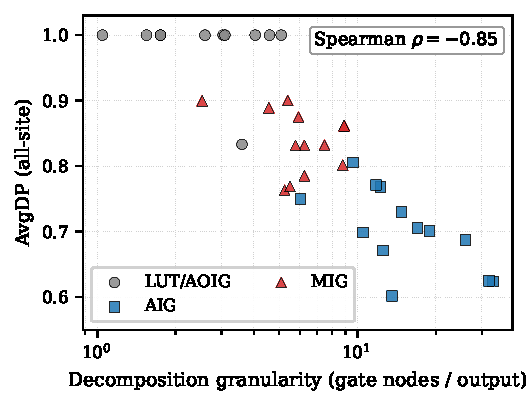
\includegraphics[width=\columnwidth]{../figures/granularity_curve}
  \caption{All-site \AvgDP{} versus decomposition granularity, measured
  as gate-output fault sites per primary output. Across LUT/AOIG, AIG,
  and MIG representations, \AvgDP{} is associated with
  representation granularity (Spearman $\rho=-0.85$ in the generated
  artifact).}
  \label{fig:granularity-curve}
\end{figure}

The mechanism is the site distribution described in
\S\ref{sec:methodology:mechanism}. A wide LUT that directly drives a
primary output contributes one output-adjacent site with high detection
probability. A decomposed-AIG or MIG contributes many interior sites, and
their effects can be masked by downstream gates. Averaging over all
sites therefore mixes a logic question with a representation-size
question. The same circuit can appear to gain or lose fault
observability depending on which baseline supplies the fault-site
population.

% =============================================================================
\subsection{Target-layer AvgDP is representation-invariant}
\label{sec:results:target-layer}

Restricting the campaign to output-driving gates removes the interior
site mix. On the evaluated circuits, target-layer \AvgDP{} is exactly
1.000 for LUT/AOIG, AIG, and MIG representations; the mean spread
across flows is 0.000. Table~\ref{tab:representation_robustness}
reports this together with the ARX/substitution \AvgBW{} ratio across
representations.

% Auto-generated by scripts/gen_reframe_tables.py
\begin{table}[t]
\centering
\caption{Granularity controls. Target-layer \AvgDP{} (output-driving gates only) is $1.000$ across all representations: the all-site difference is interior-node mix, not a changed output layer. ARX/substitution \AvgBW{} ratio is likewise stable in this benchmark, supporting an architecture-level interpretation.}
\label{tab:representation_robustness}
\begin{tabular}{lcc}
\toprule
Representation & Target-layer AvgDP & ARX/Subst.\ AvgBW \\
\midrule
LUT/AOIG & $1.000$ & $1.85\times$ \\
AIG & $1.000$ & $1.86\times$ \\
MIG & $1.000$ & $1.92\times$ \\
\bottomrule
\end{tabular}
\end{table}


This does not mean target-layer faults are the only physical faults an
attacker can induce. It means that when the target layer is held fixed,
the apparent synthesis-flow \AvgDP{} difference disappears on this
benchmark. We therefore treat all-site \AvgDP{} as a useful structural
descriptor of a netlist, but not as a representation-independent
security metric.

% =============================================================================
\subsection{ARX avalanche breadth is stable across representations}
\label{sec:results:arx}

The architecture-level \AvgBW{} result survives the granularity
controls. In the MIG flow, ARX primitives have mean \AvgBW{} $=2.056$
across Speck-32, SpecKey, and MARX-2, while the substitution-based pool
has mean \AvgBW{} $=1.082$. Every ARX value exceeds every
substitution-based value, giving a $1.90\times$ ratio
(one-sided exact Mann-Whitney $p=0.0083$). The ratio remains between
$1.85\times$ and $1.92\times$ across LUT/AOIG, AIG, and MIG
representations (Table~\ref{tab:representation_robustness}).

\begin{table}[tbp]
  \caption{Mean \AvgBW{} by cipher family (MIG flow). ARX primitives average $2.06$ output bits corrupted per detected fault versus $1.08$ for substitution-based primitives; the ratio is $1.90\times$ (Mann--Whitney $p=0.0083$). Stable across LUT/AOIG, AIG, and MIG representations (Table~\ref{tab:representation_robustness}).}
  \label{tab:arx-dichotomy}
  \centering
  \small
  \begin{tabular}{lrrcr}
    \toprule
    Family & $N$ & mean AvgBW & [min, max] & $\sigma$ \\
    \midrule
4-bit S-box & 4 & 1.013 & [1.00, 1.04] & 0.018 \\
    Subst. round & 3 & 1.173 & [1.00, 1.52] & 0.245 \\
    Permutation & 1 & 1.000 & [1.00, 1.00] & 0.000 \\
    SIMON & 2 & 1.000 & [1.00, 1.00] & 0.000 \\
    Keccak-$\chi$ & 2 & 1.000 & [1.00, 1.00] & 0.000 \\
    ARX & 3 & 2.056 & [1.71, 2.24] & 0.243 \\
    \bottomrule
  \end{tabular}
\end{table}


\begin{figure}[tbp]
  \centering
  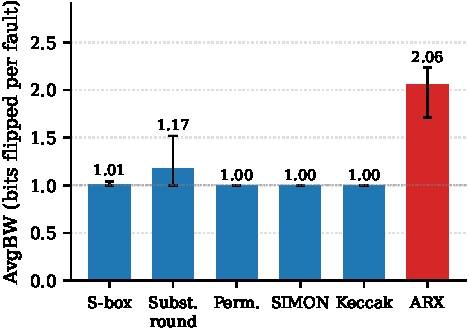
\includegraphics[width=\columnwidth]{../figures/arx_dichotomy}
  \caption{Mean \AvgBW{} by cipher architecture family in the MIG flow.
  Error bars show observed range $[\min,\max]$ over each family.}
  \label{fig:arx-dichotomy}
\end{figure}

The likely mechanism is addition-chain carry propagation: a single
internal fault in an ARX adder can change several downstream sum bits.
This is an architecture-level observation, not an exploitability claim.
Whether broader output differences help or hinder a concrete DFA depends
on the cipher's algebraic constraints and round structure.

% =============================================================================
\subsection{Higher-arity majority remains a forward path}
\label{sec:results:majn}

The granularity result tempers the interpretation of the current MIG
flow, but it does not invalidate the local masking mechanism. If a
technology provides native higher-arity majority gates, a fault entering
one input is masked whenever the remaining inputs already determine the
vote. For odd arity $n$, that masking probability is
$1-\binom{n-1}{(n-1)/2}/2^{n-1}$.

We tested direct BLIF truth-table primitives for MAJ-3, MAJ-5, and
MAJ-7 in matched synthetic chains and trees. Table~\ref{tab:majn-arity}
shows monotone \AvgDP{} reductions from MAJ-3 to MAJ-5/7, ranging from
18\% to 62\% depending on topology.

\begin{table*}[tbp]
  \caption{Synthetic MAJ-$n$ observability (chain $D{=}5$, tree $D{=}3$). \AvgDP{} drops 18--62\% from MAJ-3 to MAJ-7. $P_\text{mask}$ = theoretical per-input masking probability for odd arity $n$.}
  \label{tab:majn-arity}
  \centering
  \small
  \begin{tabular}{rrrrrrrr}
    \toprule
          &              & \multicolumn{3}{c}{Chain $D{=}5$} & \multicolumn{3}{c}{Tree $D{=}3$} \\
    \cmidrule(lr){3-5} \cmidrule(lr){6-8}
    Arity & $P_\text{mask}$ & Gates & FC\% & AvgDP & Gates & FC\% & AvgDP \\
    \midrule
3 & 0.5000 & 5 & 100.00 & 0.3875 & 13 & 100.00 & 0.3656 \\
    5 & 0.6250 & 5 & 100.00 & 0.3173 & 31 & 100.00 & 0.2057 \\
    7 & 0.6875 & 5 & 100.00 & 0.2899 & 57 & 100.00 & 0.1394 \\
    \bottomrule
  \end{tabular}
\end{table*}


This is best read as a technology hypothesis. It suggests that native MAJ-$n$
libraries could shift fault propagation if the synthesis flow preserves
MAJ-$n$ as a primitive. It does not rescue the all-site LUT-to-MIG
comparison for today's MAJ-3 decomposition flow.

\section{Discussion}
\label{sec:discussion}

% =============================================================================
\subsection{What should be reported}
\label{sec:discussion:reporting}

The main lesson is methodological. All-site fault metrics are meaningful
only together with the fault-site population they average over. Reporting
\AvgDP{} without the representation granularity can make a decomposition
look like a defense or a regression depending on the chosen baseline. A
minimum report should therefore include the number of fault sites,
fault sites per primary output, whether sites are all internal gates or a
targeted layer, and the synthesis pass that created the baseline.

For cross-representation comparisons, we recommend pairing all-site
metrics with at least one controlled metric. A decomposed-AIG baseline at comparable small-gate granularity
tests whether the effect is specific to the logic primitive rather than
to decomposition size. A target-layer metric tests whether the
attacker-facing output layer changes when interior nodes are excluded.
In our benchmark, both controls overturn the naive LUT-to-MIG
interpretation.

% =============================================================================
\subsection{What remains useful}
\label{sec:discussion:robust}

The granularity control does not make the artifact negative. It separates
three kinds of claims. First, the LUT-to-MIG \AvgDP{} reduction is a
real property of that pair of netlists, useful if a designer specifically
cares about all internal sites in those representations. Second, the
target-layer result shows that this reduction should not be promoted to a
representation-independent fault-resistance claim. Third, the ARX
\AvgBW{} result survives the controls and is therefore a stronger
design fact.

% =============================================================================
\subsection{Limits}
\label{sec:discussion:limits}

\textit{Fault model.} We model one transient \bitflip{} at one
gate-output wire. Stuck-at faults, delay faults, multi-bit faults, and
physical injection footprints may interact with representation
granularity differently.

\textit{Input model.} For large circuits we use a fixed 10,000-vector
uniform random sample; small circuits are exhaustive. An adversary who
can choose inputs may target vectors that maximize or minimize
propagation. Worst-case input search is a separate attack problem.

\textit{Target layer.} Output-driving gates are a clean controlled layer,
not a complete physical adversary model. They are useful because the
layer exists in every representation and avoids the interior-node
population shift, but other fixed layers could be studied.

\textit{Sample size.} The ARX result uses three ARX primitives and seven
substitution-based primitives. Its no-overlap pattern is strong in this
benchmark, but a wider set of addition-chain and substitution designs is
needed before treating the ratio as a general law.

\textit{End-to-end DFA.} None of the metrics directly measures key
recovery. \FCpct{}, \AvgDP{}, and \AvgBW{} describe observability and
output corruption. Algebraic usefulness of those differences remains
cipher-specific.

\section{Conclusion}
\label{sec:conclusion}

Gate-level fault observability metrics are sensitive to the granularity
of the representation being measured. On our 15-circuit cipher
benchmark, the apparent LUT/AOIG-to-MIG \AvgDP{} reduction is real for
that baseline but reverses under a decomposed-AIG control at comparable
small-gate granularity. A
target-layer campaign further shows \AvgDP{} $=1.000$ across LUT/AOIG,
AIG, and MIG representations for the evaluated circuits. The safest
conclusion is therefore not that MIG synthesis is a fault countermeasure,
but that all-site fault metrics must be reported with their
representation and site-population assumptions.

One design fact survives that control: ARX primitives produce broader
output corruption per detected fault than substitution-based primitives
across representations.
The MAJ-$n$ synthetic study points to a future technology question:
native higher-arity majority libraries may change propagation behavior,
but that must be evaluated as native MAJ-$n$, not inferred from MAJ-3
decompositions.

All measurements, scripts, and source data are included in the
accompanying reproducibility artifact.


\bibliographystyle{IEEEtran}
\bibliography{references}

\end{document}
